\section{\textit{IoT}}

\textit{Internet of Things (IoT)} adalah paradigma teknologi yang mengintegrasikan objek fisik dengan sensor, perangkat keras, dan teknologi jaringan, memungkinkan objek-objek ini untuk mengumpulkan dan bertukar data secara \textit{real-time}. Konsep ini merupakan perwujudan dari evolusi teknologi informasi, di mana objek sehari-hari bertransformasi menjadi entitas cerdas yang mampu berinteraksi dengan lingkungan sekitarnya dan jaringan digital secara lebih luas. \textit{IoT} memperkenalkan kemungkinan baru dalam otomatisasi dan pengambilan keputusan yang berbasis data, membuka jalan bagi inovasi lintas sektor \parencite{madakam2015internet}.

\begin{figure}[h]
  \centering
  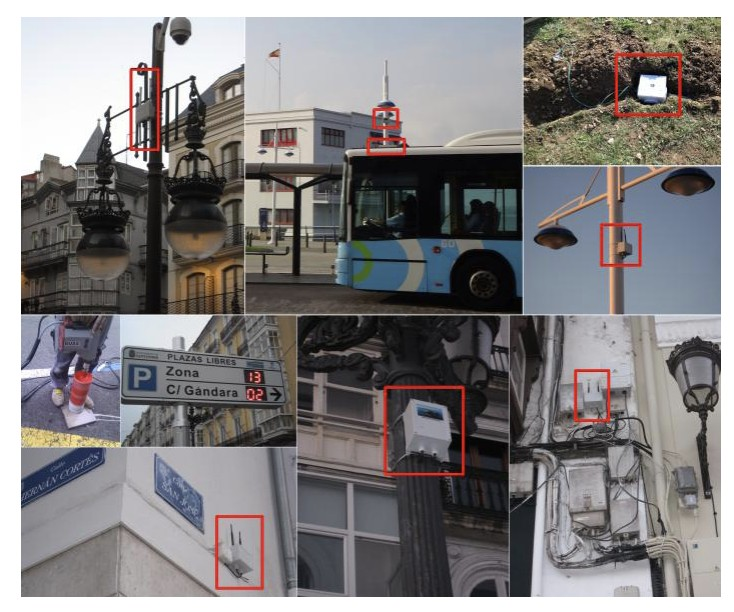
\includegraphics[width=0.8\textwidth]{resources/chapter-2/gambar-iot.jpg}
  \caption{Perangkat IoT yang terdapat pada sekitar \parencite{sotres2017practical}}
\end{figure}

\textit{IoT} memiliki aplikasi yang luas di berbagai sektor, termasuk industri, kesehatan, transportasi, dan pertanian. Dalam sektor industri, \textit{IoT} memungkinkan otomatisasi proses dan pemantauan efisiensi mesin secara real-time. Di bidang kesehatan, \textit{IoT} berkontribusi pada pengembangan perangkat medis yang terhubung untuk pemantauan kesehatan pasien. Dalam transportasi, \textit{IoT} mendukung pengembangan kendaraan otonom dan sistem manajemen lalu lintas cerdas. Di sektor pertanian, \textit{IoT} digunakan untuk memantau kondisi tanah dan iklim, membantu petani dalam pengambilan keputusan.

Dalam penerapannya \textit{IoT} dapat dibagi menjadi tiga lapisan, yaitu lapisan persepsi, lapisan jaringan, dan lapisan aplikasi secara berurutan. Lapisan persepsi bertanggung jawab atas pengumpulan data dalam \textit{IoT}. Lapisan ini terdiri dari berbagai jenis sensor, seperti sensor suhu, sensor kelembaban, RFID, kamera, GPS, dan sebagainya. Lapisan jaringan terdiri dari berbagai jenis jaringan, seperti internet, jaringan komunikasi 2G dan 3G, serta jaringan siaran. Lapisan jaringan terutama digunakan untuk mengumpulkan data dari lapisan persepsi dan memproses data tersebut untuk lapisan aplikasi. Terakhir yaitu Lapisan aplikasi, Lapisan ini adalah antarmuka antara pengguna dan \textit{IoT}. Banyak aplikasi, termasuk logistik, rantai pasokan, pertanian, industri, keamanan publik, pengelolaan perkotaan, telemedis, rumah pintar, transportasi pintar, dan pemantauan lingkungan, diaktifkan melalui \textit{IoT} \parencite{SmartHomeSystemBasedOnIoTTechnologies}.

Seiring bertambahnya jumlah perangkat \textit{IoT} perlu dibuat suatu cara agar sistem \textit{scalable}. \textit{Device discovery} merupakan salah satu masalah yang perlu diatasi untuk membuat sistem \textit{IoT} yang \textit{scalable} karena dapat meningkatkan \textit{quality of service} sehingga meningkatkan availabilty \parencite{DeviceDiscovery}. Tidak hanya itu, banyak munculnya perangkat \textit{IoT} baru yang memerlukan \textit{update} secara berkala menimbulkan masalah baru yaitu sulitnya untuk melakukan \textit{update} untuk setiap perangkat yang ada apabila jumlahnya semakin meningkat sehingga peran \textit{remote deployment} menjadi sangat penting dalam menyelesaikan masalah ini \parencite{RemoteDeployment}.